
\subsection{Dataflow Diagram Level 0}
\begin{figure}[h]
    \centering
    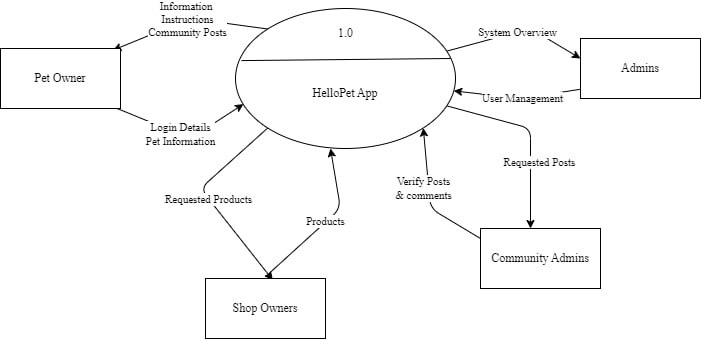
\includegraphics[width= 5in ]{img/dfd_0.jpg}
    \caption[DFD Level 0]{DFD Level 0}
    \label{fig:dfd-level0}
\end{figure}

\justify
A Data Flow Diagram (DFD) Level 0 provides a high-level overview of the system and its interactions with external entities. In your case, the system is the "HelloPet" app, and the external entities are admins, community admins, shop, and pet owners.

    \noindent\textbf{HelloPet App (System)}\\
        This is the main system under consideration (HelloPet app).
        It interacts with various external entities to fulfill its functionalities.

    \noindent\textbf{Admins}\\
        Admins are responsible for user management and have access to a system overview.
        They provide administrative services related to the management of users within the HelloPet app.
        They can view a comprehensive overview of the system.

    \noindent\textbf{Community Admins}\\
        Community admins are responsible for managing community-related activities.
        They handle requested posts from users.
        They verify and manage posts and comments within the community.

        \noindent\textbf{Shop}\\
        The shop entity deals with products and product-related services.
        It manages the available products and handles requests for new products.
\newpage
        \noindent\textbf{Pet Owners}\\
        Pet owners are the end-users of the HelloPet app.
        They provide login details to access the app.
        They submit and manage pet information, including details and instructions related to their pets.

    \noindent Hence, the data flow diagram indicates the visualization of system with its input feed to the system by User.\\


    \subsection{DFD Level 1}
    \vspace{2cm}
    \begin{figure}[H]
    \centering
    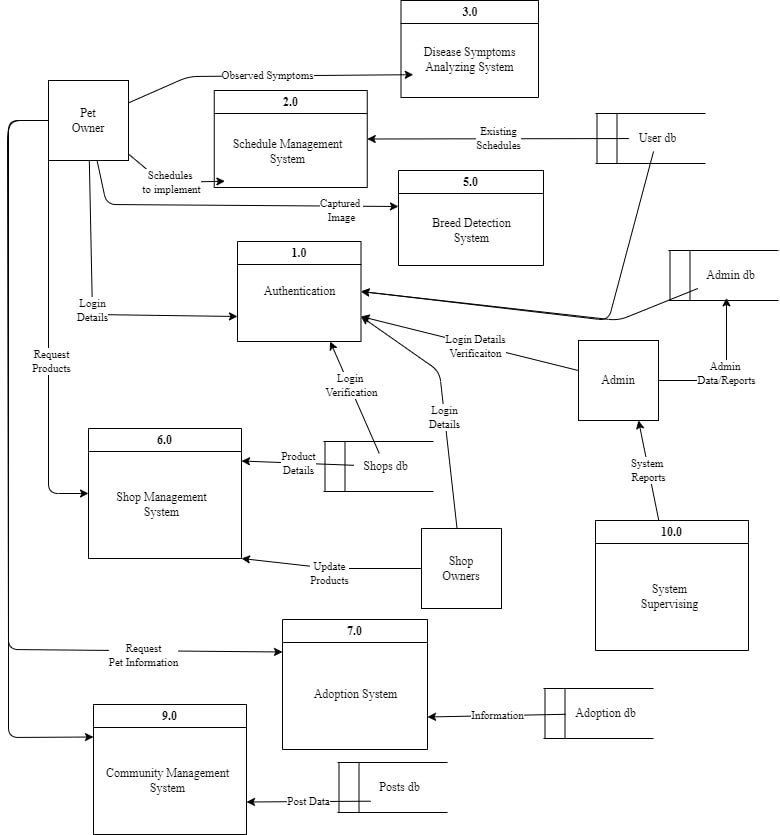
\includegraphics[width=0.95\linewidth]{img/dfd_1.jpg}
    \caption[DFD Level 1]{DFD Level 1}
    \label{fig:dfd-level1}
    \end{figure}
    \textbf{Schedule Management System}\\
        Allows pet owners to observe symptoms and schedule appointments.
        Interacts with the User Database to store appointment details.
    
    \textbf{Breed Detection System}\\
        Captures images for breed detection.
        Performs breed analysis.
    
    \textbf{Authentication System}\\
        Handles login details and user verification.
        Connects to the Admin Database for admin logins.
    
    \textbf{Shop Management System}\\
        Manages product details (e.g., pet supplies, accessories).
        Interacts with Shop Owners for updates.
    
    \textbf{Schedule Management System}\\
        Allows pet owners to observe symptoms and schedule appointments.
        Interacts with the User Database to store appointment details.
    
    \textbf{Breed Detection System}\\
        Captures images for breed detection.
        Performs breed analysis.
    
    \textbf{Authentication System}\\
        Handles login details and user verification.
        Connects to the Admin Database for admin logins.
    
    \textbf{Shop Management System}\\
        Manages product details (e.g., pet supplies, accessories).
        Interacts with Shop Owners for updates.
    
    \textbf{Adoption System}\\
        Handles pet information requests.
        Connects to the Adoption Database.
    
    \textbf{Community Management System}\\
        Manages post data (e.g., pet-related discussions, tips).
        Allows users to engage with each other.
        Handles pet information requests.
        Connects to the Adoption Database.
    
    \textbf{Community Management System}\\
        Manages post data (e.g., pet-related discussions, tips).
        Allows users to engage with each other.